\documentclass{article}
\usepackage[UTF8]{ctex} % 添加ctex宏包以支持中文编译
\usepackage{graphicx} % Required for inserting images

\title{DCT-REM}
\author{Yongjian Zhao}
\date{March 2026}
\usepackage{algorithmic}
\usepackage{algorithm}
\usepackage{array}
\usepackage[caption=false,font=normalsize,labelfont=sf,textfont=sf]{subfig}
\usepackage{amsmath,amssymb,amsfonts}

% ---------- 版面与图形 ----------

\usepackage{graphicx}
\usepackage{adjustbox}
\usepackage{textcomp}
\usepackage{siunitx}
\usepackage{textcomp}
\usepackage{stfloats}
\usepackage{url}
\usepackage{verbatim}

\usepackage{array,booktabs,tabularx}
\usepackage{multirow}
\usepackage{hyperref}
\usepackage{adjustbox}
\newcommand{\cmark}{\ding{51}}  % ✓
\newcommand{\xmark}{\ding{55}}  % ✗
\usepackage{pifont}                  % \ding symbols
\newcommand{\fstar}{\ding{72}}       % filled star
\newcommand{\hstar}{\ding{73}}       % hollow star
\newcolumntype{C}[1]{>{\centering\arraybackslash}p{#1}}
\renewcommand{\arraystretch}{1.15}

% ---------- 颜色与引用 ----------
\usepackage{xcolor}                              % ← 必须先加载
\definecolor{labelblue}{RGB}{0,0,180}
\definecolor{numberblue}{RGB}{0,0,180}

\makeatletter                                     % ← 解除 natbib 钩子
\let\NAT@parse\undefined
\makeatother

\usepackage[capitalize]{cleveref}                % ← 后 cleveref
\usepackage[numbers]{natbib}

% ===== cleveref 样式统一 =====
% equation
\crefname   {equation}{\textcolor{labelblue}{公式}}{\textcolor{labelblue}{公式}}
\Crefname   {equation}{\textcolor{labelblue}{公式}}{\textcolor{labelblue}{公式}}
\creflabelformat{equation}{\textcolor{numberblue}{(#2#1#3)}}

% figure
\crefname   {figure}  {\textcolor{labelblue}{图}}     {\textcolor{labelblue}{图}}
\Crefname   {figure}  {\textcolor{labelblue}{图}}     {\textcolor{labelblue}{图}}
\creflabelformat{figure}{\textcolor{numberblue}{#2#1#3}}

% table
\crefname   {table}   {\textcolor{labelblue}{表}}   {\textcolor{labelblue}{表}}
\Crefname   {table}   {\textcolor{labelblue}{表}}   {\textcolor{labelblue}{表}}
\creflabelformat{table}{\textcolor{numberblue}{#2#1#3}}

% algorithm
\crefname   {algorithm}{\textcolor{labelblue}{算法}}{\textcolor{labelblue}{算法}}
\Crefname   {algorithm}{\textcolor{labelblue}{算法}}{\textcolor{labelblue}{算法}}
\creflabelformat{algorithm}{\textcolor{numberblue}{#2#1#3}}

% ---------- 其他 ----------
\hyphenation{op-tical net-works semi-conduc-tor IEEE-Xplore}

\begin{document}

\maketitle
\section{双传感器混合 6-DoF 伺服框架}
\label{sec:6dof_framework}
针对空间站环境下的特定血管平面追踪任务 ，本文采用自主设计的机器人光声层析（PAT）系统。该系统将 PAT 探头集成于机械臂末端，用于获取局部血管的高分辨率横截面图像 。由于该任务涉及复杂的六自由度（6-DoF）空间追踪，本文提出了一种基于“宏观引导-微观伺服”的混合控制策略 。

在追踪初始阶段，当目标尚未进入光声成像视野时，系统利用末端搭载的深度相机（Depth Camera）提供宏观全局视野，引导机械臂向目标区域逼近。该过程受两个关键空间条件约束：首先，探头末端需与皮肤表面保持特定的工作距离 $d^*$，该距离由探头的合成焦距严格标定；其次，探头需被引导至目标血管的宏观邻域内 。

\begin{table}[htbp]
    \centering
    \caption{混合系统中的自由度解耦与反馈映射 }
    \label{tab:dof_decoupling}
    \begin{tabularx}{\columnwidth}{XXXX}
        \toprule
        \textbf{DoF 分量} & \textbf{伺服类型} & \textbf{反馈信号来源} & \textbf{控制目标} \\
        \midrule
        $v_x, v_y$ & IBVS & 光声 DCT 特征 $\mathbf{s}(\mathbf{I})$ & 面内横截面平移对齐 \\
        $\omega_z$ & IBVS & 光声 DCT 特征 $\mathbf{s}(\mathbf{I})$ & 面内横截面旋转对齐 \\
        $v_z$ & PBVS & 深度相机 $d$ & 维持恒定工作距离 $d^*$ \\
        $\omega_x, \omega_y$ & PBVS & 深度相机法向量 $\mathbf{n}$ & 面外姿态对齐 \\
        \bottomrule
    \end{tabularx}
\end{table}

当完成初始定位且光声图像成功显现后，系统无缝切换至混合视觉伺服阶段 。为保证所有光声图像均在同一高度平面内采集，深度相机将在全过程中持续主导 $Z$ 轴方向的位置伺服，以维持恒定的工作距离 $d^*$ 。具体而言，系统采用了如\cref{tab:dof_decoupling}所示的解耦策略：面内分量（$v_x, v_y, \omega_z$）由基于光声 DCT 特征 $\mathbf{s}(\mathbf{I})$ 的基于图像的视觉伺服（IBVS）控制；面外分量（$\omega_x, \omega_y, v_z$）则由基于深度信息的基于位置的视觉伺服（PBVS）闭环接管。

\subsection{光声平面外的位置伺服理论推导}
\label{sec:out_of_plane}
在光声成像中，单一的二维切片无法提供完整的光声平面外运动观测 。为此，本系统集成深度相机以接管面外子空间（Out-of-plane subspace）的控制，包含沿 $Z$ 轴的平移以及绕 $X, Y$ 轴的旋转 。

设 $d$ 为深度相机实测距离，$\mathbf{n} = [n_x, n_y, n_z]^\top$ 为当前观测到的目标表面单位法向量 。为了维持探头成像平面平行于皮肤表面（从而使声束垂直于血管平面截断）并保持恒定距离，定义期望距离为 $d^*$，期望单位法向量为 $\mathbf{n}^* = [0, 0, 1]^\top$ 。

由此，定义沿 $Z$ 轴的距离误差 $e_d$ 为：
\begin{equation}
e_d = d - d^*
\end{equation}

对于光声平面外姿态对齐，系统根据轴角表示法推导姿态误差 $\mathbf{e}_{out}$。为了消除向量模长对控制增益的影响，利用单位法向量的叉乘定义误差：

\begin{equation}
\mathbf{e}_{out} = \mathbf{n} \times \mathbf{n}^* = \begin{bmatrix} n_x \\ n_y \\ n_z \end{bmatrix} \times \begin{bmatrix} 0 \\ 0 \\ 1 \end{bmatrix} = \begin{bmatrix} n_y \\ -n_x \\ 0 \end{bmatrix}
\end{equation}

由于偏航角（$\omega_z$）已由面内特征解耦控制，面外伺服仅提取 $\mathbf{e}_{out}$ 的前两项 。基于位置的视觉伺服（PBVS）导出的面外速度指令 $\mathbf{v}_{out} = [v_z, \omega_x, \omega_y]^\top$ 设计为 ：
\begin{equation}
\mathbf{v}_{out} = -\lambda_{out} \begin{bmatrix} e_d \\ n_y \\ -n_x \end{bmatrix}
\end{equation}
其中，$\lambda_{out} > 0$ 为调节面外收敛速度的增益系数 。


\subsection{平面伺服框架：基于DCT的伺服控制算法设计}
\label{sec:algorithm}

本文提出了一种基于离散余弦变换（DCT）的视觉伺服框架，以在特定的光声（PA）成像约束下鲁棒地提取和控制视觉特征。本节首先简要回顾了标准频谱变换的集成，随后详细阐述了我们的核心创新：针对光声成像几何特性优化的频域交互矩阵公式，并最终推导出一个混合 6-DoF 双传感器伺服框架——该框架利用 Intel Depth camera 深度相机实现了鲁棒的光声平面外（out-of-plane）运动补偿。

\subsubsection{频谱特征表示}
\label{sec:Spectral_Feature_Representation}

传统的基于图像的视觉伺服（IBVS）通过最小化当前传感器数据与期望目标配置之间的特征空间差异来调节机器人的运动。然而，传统的IBVS依赖于空间像素强度，当应用于医学超声和光声成像时，其表现出极高的噪声敏感性，且收敛域受到严重限制。由于受限于激光的帧率和非平稳的电磁干扰，光声视觉伺服面临的挑战进一步加剧。

为了克服这些特定模态的限制，我们的方法避开了空间强度特征，直接将光声感兴趣区域（ROI）转换至频域。利用成熟的二维离散余弦变换（DCT）\cite{ahmed2006discrete}，我们将空间强度映射为频率系数矩阵。通过采用标准的Z字形扫描协议（如图\Cref{fig:feature_construction}(c)所示），我们优先保留低频分量，从而提取出紧凑的视觉特征向量 \(\boldsymbol{s}(u,v) \in \mathbb{R}^K\)。这种频谱截断本质上充当了一个低通滤波器（如图\Cref{fig:DCT_transform}所示），在保留宏观血管拓扑结构的同时，滤除了原始光声信号中特征性的高频干扰。


Consider a photoacoustic image region of interest (ROI) represented by pixel intensities \(\boldsymbol{I}(x, y)\) with dimensions \(M \times N\). The two-dimensional DCT-II transform maps this spatial-domain representation to the frequency domain through \cite{ahmed2006discrete}:
\begin{equation}
\boldsymbol{F}_{uv} = \sum_{y=0}^{N-1} \sum_{x=0}^{M-1} \phi_{uv}(x,y)\,\boldsymbol{I}(x,y),
\label{2D-DCT-equation}
\end{equation}
\begin{figure}[!htb]
    \centering
    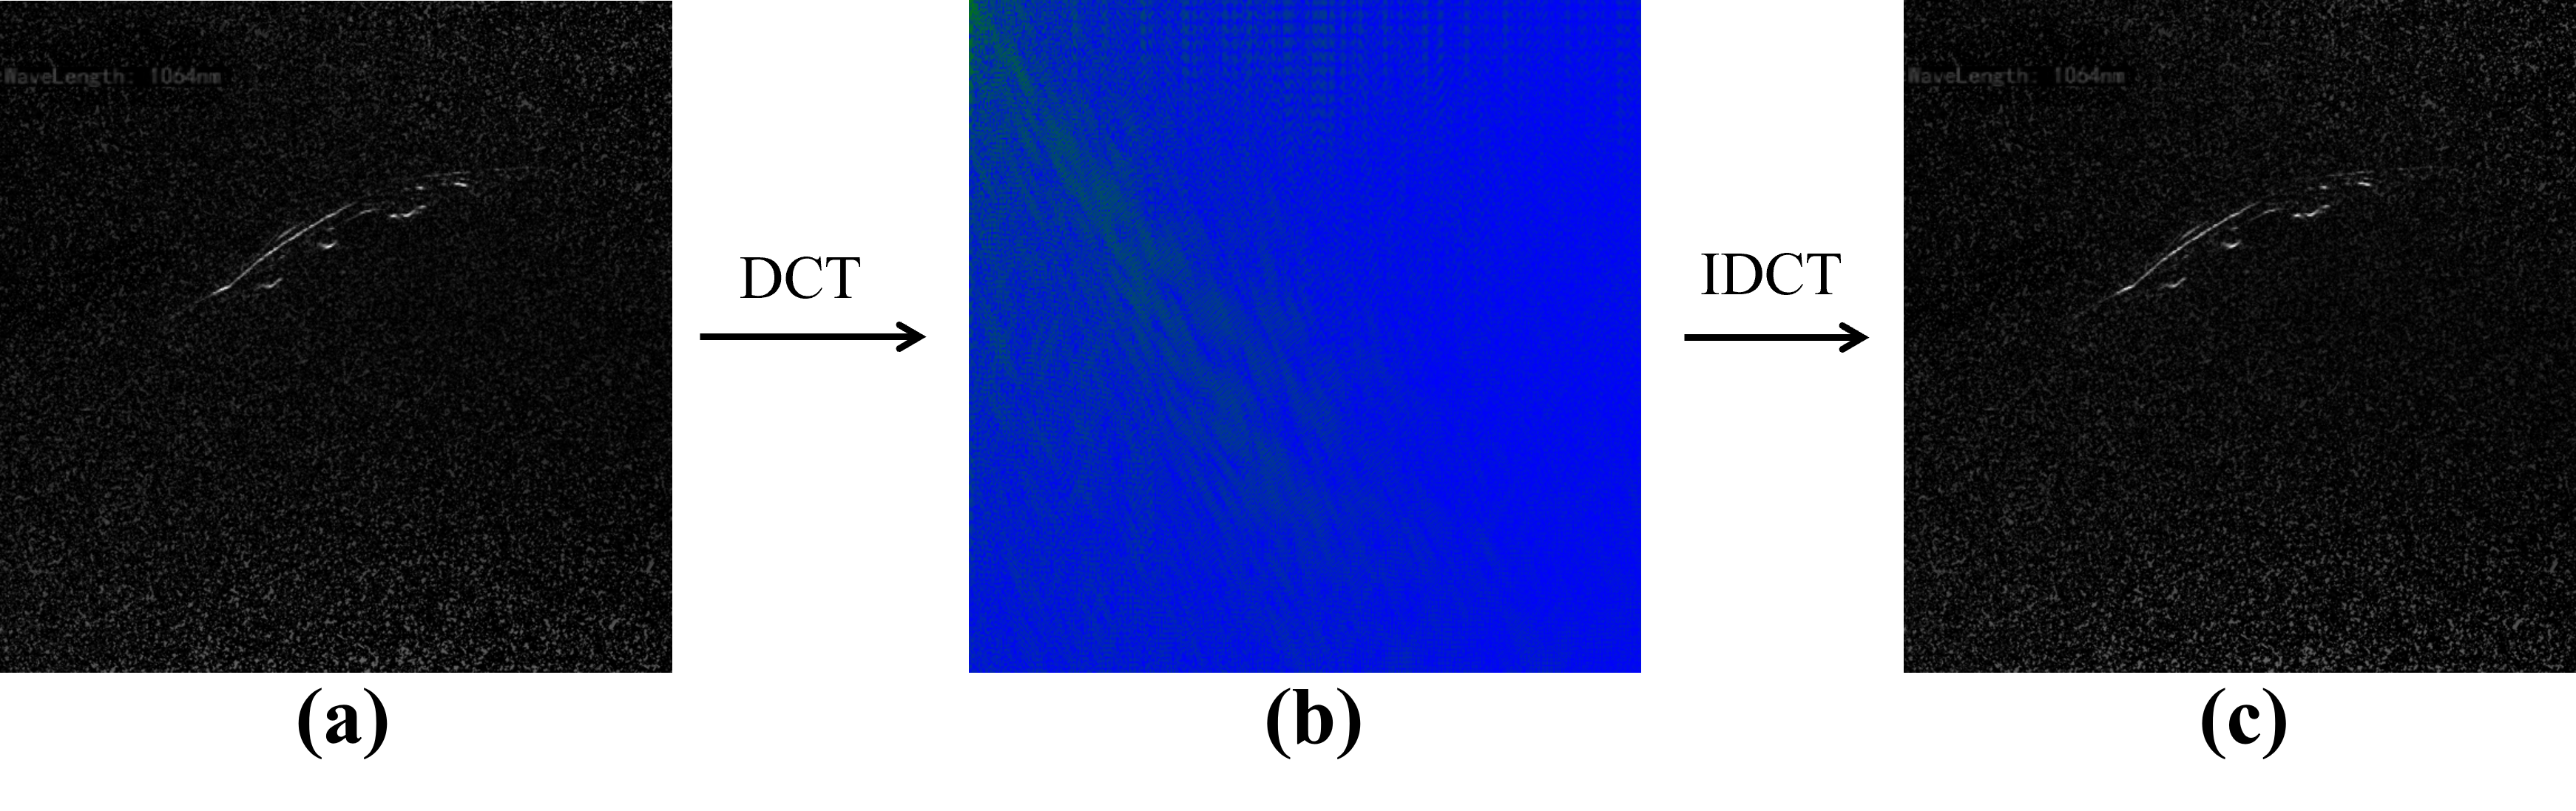
\includegraphics[width=\columnwidth]{graph/IDCT_new.png}
    \caption{Spectral decomposition and reconstruction via Discrete Cosine Transform: 
    (a) Original spatial-domain vascular image \(\boldsymbol{I}(x, y)\), 
    (b) Frequency-domain coefficient matrix \(\boldsymbol{F}(u, v)\) showing characteristic energy compaction in low-frequency quadrant, 
    (c) Perfect reconstruction through IDCT validating transformation integrity and noise preservation properties}
    \label{fig:DCT_transform}
\end{figure}


其中，$\phi_{uv}(x,y)$是基函数，The transformation can be expressed in matrix formulation as:
\begin{equation}
\boldsymbol{F} = \boldsymbol{C}_M \boldsymbol{I} \boldsymbol{C}_N^T,
\end{equation}
where \(\boldsymbol{C}_M\) and \(\boldsymbol{C}_N\) are orthogonal transform matrices of sizes \(M\) and \(N\) respectively. 

This coordinate transformation preserves all image information, enabling perfect reconstruction via the inverse DCT (IDCT) as demonstrated in \Cref{fig:DCT_transform}(c). While IDCT serves primarily for visualization in this context, partial coefficient reconstruction introduces approximation errors \cite{kleinman1962nonlinear} (see \Cref{fig:spectral_reconstruction}(c)). The DCT coefficients \(\boldsymbol{F}(u,v)\) therefore constitute effective visual features, replacing raw pixel intensities in the servo framework.

\begin{figure*}[htbp]
    \centering
    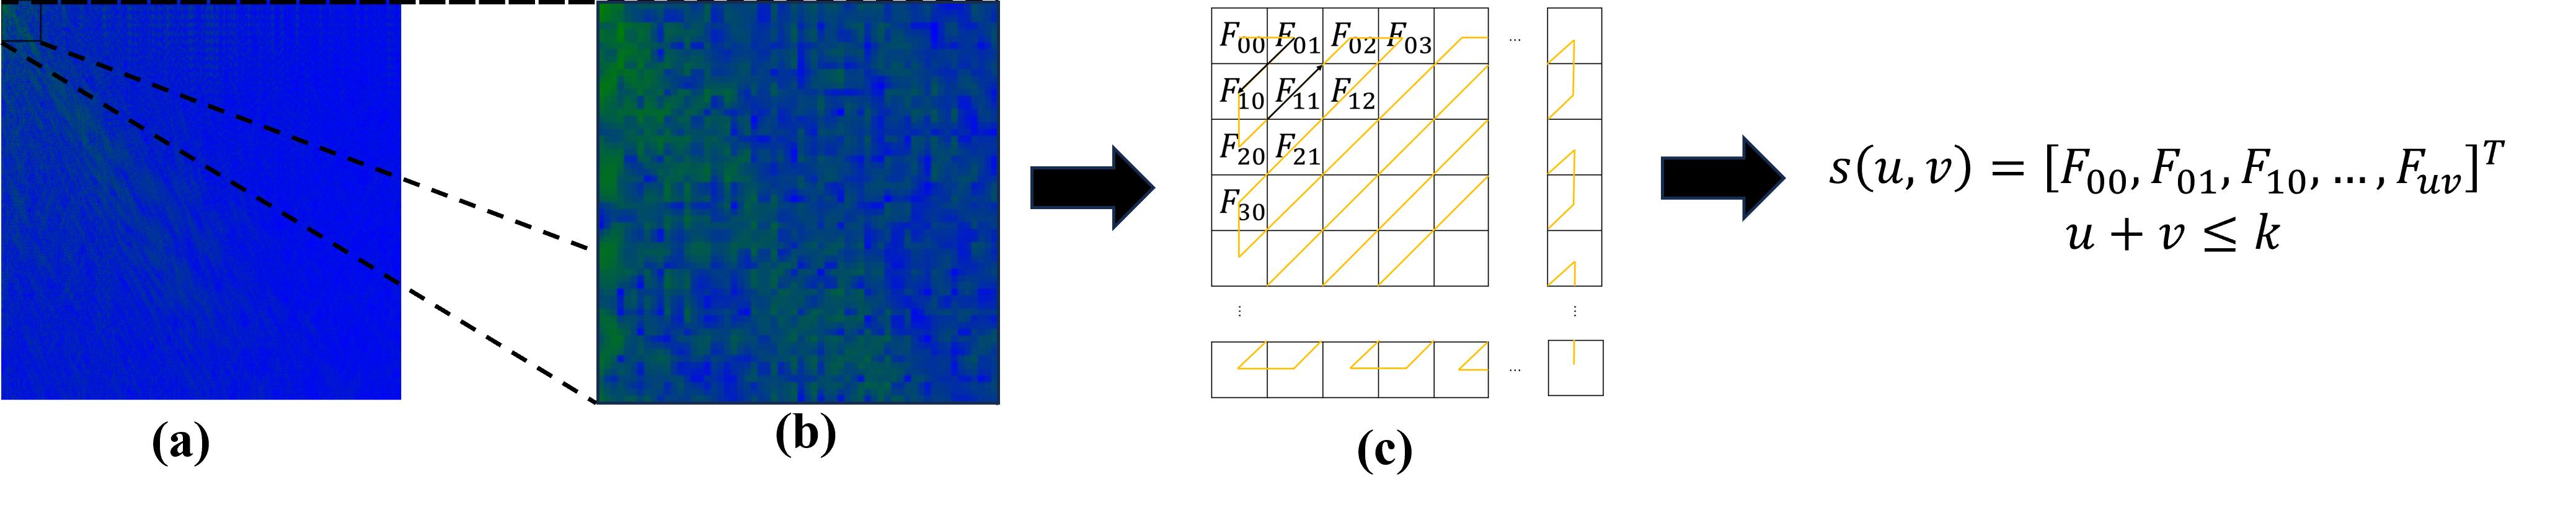
\includegraphics[width=\columnwidth]{graph/spatial calibration.png}
    \caption{Frequency-domain visual feature construction methodology: 
    (a) 2D DCT coefficient spectrum showing spectral energy concentration in low-frequency quadrant (\(u,v < 5\)), 
    (b) Magnified visualization of low-frequency region (\(0 \leq u,v \leq 15\)) demonstrating energy compaction property, 
    (c) Zigzag scanning protocol selecting coefficients satisfying \(u + v \leq k\) to construct compressed feature vector:  
    \(\boldsymbol{s}(u,v) = [F_{00}, F_{01}, F_{10}, \dots, F_{uv}]^\top \in \mathbb{R}^K\)}
    \label{fig:feature_construction}
\end{figure*}

接下来，我们建立了一种利用 DCT 系数的紧凑特征表示方法。对于一个频率索引为 \(u \in [0, M-1]\)、\(v \in [0, N-1]\) 的 \(M \times N\) 数字图像 \(\boldsymbol{I}(x,y)\)，根据 \Cref{2D-DCT-equation} 计算第 \(K\) 阶矩系数（其中 \(K = u + v\)）。视觉特征向量构建如下：
\begin{equation}
\boldsymbol{s}(u, v) = \left[F_{00}, F_{01}, F_{10}, \dots, F_{uv}\right]^T, \quad u + v \le K,
\label{visual feature}
\end{equation}
其中每个 \(F_{uv}\) 均由 DCT 矩阵计算得出。这种基于系数的表示方法在保持视觉识别和跟踪应用判别力的同时，提供了高效的特征编码。

\subsection{DCT 系数选择的最优排序 和 动态特征阶数计算}
\label{secdynamic coeff}

DCT 系数通过曲折扫描（Zigzag）进行系统排序（见 \Cref{fig:feature_construction}(c)）。具体而言，该过程始于由水平 ($u$) 和垂直 ($v$) 空间频率索引的系数矩阵，沿 $F_{00}$ 开始的遍历路径进行（方向箭头指示扫描序列：$F_{00} \rightarrow F_{01} \rightarrow F_{10} \rightarrow \cdots$），通过提取满足 $u + v \leq k$ 的系数（阴影区域）构建特征向量，得到 $\boldsymbol{s}(u,v) = [F_{00}, F_{01}, \dots, F_{uv}]^\top \in \mathbb{R}^K$。这种扫描方式优先保留了携带主要能量的低频分量，同时将接近零的高频分量置于末尾，从而实现了特征的有效压缩。对于给定的相机位姿 \(\boldsymbol{r}\)，视觉特征向量 \(\boldsymbol{s}(\boldsymbol{r})\) 即由图像 \(\boldsymbol{I}(\boldsymbol{r})\) 经此模式提取的 DCT 系数组成。


保留前 \(K\) 个按曲折顺序排列的系数构成了光谱低通滤波，如 \Cref{fig:DCT_transform}(c) 中有限系数 IDCT 重建所示。交互矩阵 \(\boldsymbol{L}_s\) 的计算方法与 \Cref{L_S} 类似，但被限制在 \(K\) 维曲折选择子空间内，从而将维度从 \(N^2 \times 6\) 降低到 \(K \times 6\)。


按照正交矩阵排序，通过 \Cref{visual feature} 提取视觉伺服（VS）特征。较低的矩阵阶数强调全局图像结构，增强了噪声抑制和压缩效率 \cite{chen2024direct}。然而，这种粗糙的表示会损害细微细节的分辨率，增加伺服过程中陷入局部极小值的可能性。相反，较高的阶数能够捕获更精细的图像细节以提高终端收敛精度，但由于过度关注微观变化，会产生计算延迟，于是我们需要建立一个动态选择DCT 系数\(K\)的选择机制，以平衡计算效率和高图像分辨率之间的关系。本文引入了一种自适应阶数选择策略。该策略的核心逻辑在于：根据当前特征误差的收敛状态，动态调整保留的 DCT 系数数量 $K$ 。

定义当前特征向量与期望特征向量之间的均方误差（MSE）为 $\bar{e}_s$。为了实现从“粗略快速跟踪”到“高精度对准”的平滑切换，令系数数量 $K$ 随误差有界单调进行动态缩放 ：
\begin{equation}
K = round(\left(K_{\max} - K_{\min}\right) \eta + K_{\min}), \quad \eta \in [0, 1], \quad K \in \mathbb{N},
\end{equation}
其中，$K_{max}$ 和 $K_{min}$ 分别代表预设的最高和最低频谱截断阶数。自适应调节因子 $\eta$ 由初始误差 $\bar{e}_s^0$ 和当前误差 $\bar{e}_s$ 共同定义：

\begin{equation}
\eta = \frac{\bar{e}_s^0}{\bar{e}_s^0 + \lambda_\eta \, \bar{e}_s}.
\end{equation}

Here, \(\bar{e}_s\) and \(\bar{e}_s^0\) denote the mean squared errors (MSE) for current and initial features respectively:
\begin{equation}
\bar{e}_s = \frac{1}{K} \sum_u \sum_v \left(\boldsymbol{s}(u, v) - \boldsymbol{s}^{*}(u, v)\right)^2,
\end{equation}
\begin{equation}
\bar{e}_s^0 = \frac{1}{K} \sum_u \sum_v \left(\boldsymbol{s}_0(u, v) - \boldsymbol{s}^{*}(u, v)\right)^2.
\end{equation}

Assuming exponential error decay (\(\bar{e}_s = \bar{e}_s^0 e^{-\lambda_0 t}\)) per ideal control behavior, \Cref{dynamic coefficients} simplifies to:
\begin{equation}
\eta = \frac{1}{1 + \lambda_\eta e^{-\lambda_0 t}}.
\end{equation}
Coefficient count \(K\) is then computed via \Cref{dynamic coefficients of k}, with boundary selection methodology further elaborated in \Cref{sec:mask}.


此处 $\lambda_{\eta} > 0$ 为缩放增益。当系统处于搜索初期（$\bar{e}_s$ 较大）时，$\eta$ 较小，系统仅保留极少数低频系数以获得极大的收敛域并过滤干扰；随着误差减小，$\eta$ 趋近于 1，$K$ 自动增加以引入更多高频解剖细节，确保对准精度。

\subsubsection{面向光声优化的交互矩阵构建}
\label{sec:PA-Optimized_Interaction_Matrix}

传统的IBVS依赖于通过针孔模型从三维场景投影到二维平面的相机数据，而光声视觉伺服则在完全不同的图像形成机制下运行。光声图像代表的是二维横截面视图；只有当解剖结构与特定的光声声束平面相交时，才能捕获到相关特征,光声图像可以采用正交比例缩放模型，即可近似为平面内的仿射/比例映射 \cite{nadeau2013intensity}。

我们将成像平面（探头平面）定义为坐标系 \(\mathcal{F}_p\)，其原点位于图像中心 \(P(u_0, v_0)\)。在此统一坐标系下，\(Z_p\)轴与光声传播方向（深度方向）对齐，而图像平面由\(X_p\)和\(Y_p\)轴构成。在此几何结构下，物理点 \(\mathbf{P} = (X_p, Y_p, 0)^\top\) 通过内部比例因子 \(\alpha_u\) 和 \(\alpha_v\) 映射到像素坐标 \((u, v)\)：
\begin{equation}
\begin{cases}
u = \alpha_u X_p + u_0 \\[2mm]
v = \alpha_v Y_p + v_0
\end{cases}
\end{equation}
其中比例因子 $(\alpha_u, \alpha_v)$ 将空间坐标转换为像素坐标。它们的倒数 $(\delta_x = 1/\alpha_u, \delta_y = 1/\alpha_v)$ 构成了探头的内参。结合世界坐标系 $\mathcal{F}_w$ 中的外参位姿（见 \Cref{fig:coordinate_systems}），该几何模型能够通过标定后的变换实现 3D 坐标测量 \cite{mercier2005review}。

在环境静止及光声反射率恒定的假设下，我们对频域特征进行时间求导，从而将微分 $\dot{\boldsymbol{s}}_{(u,v)}$ 映射到六自由度（6-DoF）探头速度 $\mathbf{v}_c \in \mathbb{R}^6$：
\begin{equation}
\dot{\boldsymbol{s}}_{(u,v)} = \boldsymbol{L}_{\boldsymbol{s}_{(u,v)}} \mathbf{v}_c
\label{eq:s=LV}
\end{equation}

在环境静止假设 (H1) 和恒定光声反射假设 (H2) \cite{nadeau2013intensity} 下，基于强度的伺服控制允许直接从像素强度推导特征。传感器速度指令变为：
\begin{equation}
\mathbf{v}_c = -\lambda \boldsymbol{L}^{+}_{\boldsymbol{s}_{(u,v)}} (\boldsymbol{s}_{(u,v)} - \boldsymbol{s}^*_{(u,v)})
\end{equation}
其中 $\boldsymbol{s}_{(u,v)}$ 和 $\boldsymbol{s}^*_{(u,v)}$ 分别表示当前的和目标的 DCT 特征。

应用一阶泰勒近似：
\begin{equation}
\dot{\boldsymbol{s}}_{(u,v)} = \nabla \boldsymbol{s}_{(u,v)} \cdot \dot{\boldsymbol{x}}_P
\end{equation}
其中特征空间梯度为 $\nabla \boldsymbol{s}_{(u,v)} = [\nabla s_x, \nabla s_y, \nabla s_z]$ ，点运动方程为：
\begin{equation}
\dot{\boldsymbol{x}}_P = \left[ \boldsymbol{I}_3 \quad -[\boldsymbol{x}_P]_\times \right] \dot{\mathbf{v}}_c
\end{equation}
其中 $\dot{\mathbf{v}}_c$ 代表探头相对于世界坐标系的速度。

由此得到的系数 $(u,v)$ 的交互矩阵为：
\begin{equation} \label{eq:L_s_uv}
	\begin{aligned}
		\boldsymbol{L}_{s_{(u,v)}} = 
		& \left[\nabla s_x \quad \nabla s_y \quad \nabla s_z \quad y\nabla s_z \right. \\
		&\left.\; -x\nabla s_z \quad x\nabla s_y - y\nabla s_x\right]
	\end{aligned}
\end{equation}

完整的交互矩阵汇总了所有保留的系数：
\begin{equation}
\boldsymbol{L}_s = 
\begin{bmatrix}
\boldsymbol{L}_{s_{(1,1)}}^\top & \cdots & \boldsymbol{L}_{s_{(m,n)}}^\top
\end{bmatrix}^\top
\label{L_S}
\end{equation}

\subsubsection{光度视觉伺服与基于 DCT 的视觉伺服控制律的对比公式化}
\label{comparative Formulation}
对 \Cref{2D-DCT-equation} 关于时间求导得：
\begin{equation}
\dot{\boldsymbol{F}}_{uv} = \sum_{x,y} \phi_{uv}(x,y) \, \dot{\boldsymbol{I}}(x,y).
\label{eq:dotF}
\end{equation}

在假设强度变化完全由传感器运动引起的情况下，图像亮度恒定约束提供：
\begin{equation}
\dot{\boldsymbol{I}}(x,y) = \nabla \boldsymbol{I}(x,y) \cdot \dot{\mathbf{v}}_p,
\label{eq:dIdt}
\end{equation}
其中 $\nabla \boldsymbol{I} = \left[ \partial_x \boldsymbol{I}, \partial_y \boldsymbol{I}, \partial_z \boldsymbol{I} \right]^\top$ 表示空间强度梯度，$\dot{\mathbf{v}}_p$ 表示投影到像素 $(x,y)$ 的点的瞬时 3D 速度 \cite{chaumette2006visual}。

采用针孔（一阶）投影模型：
\begin{equation}
\dot{\mathbf{v}}_p = \mathbf{J}(x,y) \, \mathbf{v}_c,
\label{eq:Jpixel}
\end{equation}
配合标准图像雅可比矩阵：
\begin{equation}
\begin{aligned}
\mathbf{J}(x,y) &=
\begin{bmatrix}
-\dfrac{1}{Z} & 0 & \dfrac{x}{Z} & xy & -(1+x^{2}) & y \\
0 & -\dfrac{1}{Z} & \dfrac{y}{Z} & 1+y^{2} & -xy & -x
\end{bmatrix} \\[1em]
\mathbf{v}_c &=
\begin{bmatrix}
v_x, v_y, v_z, \omega_x, \omega_y, \omega_z
\end{bmatrix}^\top = \begin{bmatrix} \mathbf{v}, \boldsymbol{\omega} \end{bmatrix}^\top
\end{aligned}
\label{eq:image_jacobian}
\end{equation}
其中 $Z$ 表示场景深度（在单平面光声成像中被视为常数）。

将 \Cref{eq:dIdt} 和 \Cref{eq:Jpixel} 代入 \Cref{eq:dotF} 得：
\begin{equation}
\dot{\boldsymbol{F}}_{(uv)} 
= \underbrace{\sum_{x,y} \phi_{uv}(x,y) \, \nabla \boldsymbol{I}(x,y) \, \mathbf{J}(x,y)}_{\boldsymbol{L}_{\boldsymbol{F}_{uv}}} \, \mathbf{v}_c,
\label{eq:LFuv}
\end{equation}
    其中 $\boldsymbol{L}_{F_{uv}} \in \mathbb{R}^{1 \times 6}$ 构成了系数 $\boldsymbol{F}_{uv}$ 的交互行向量，显式表达为：

\begin{equation} \label{eq:LFuv_explicit}
\begin{aligned}
	\boldsymbol{L}_{F_{uv}} = 
	&\left[
		\nabla_x \boldsymbol{F}_{uv}, \quad 
		\nabla_y \boldsymbol{F}_{uv}, \quad  
		\nabla_z \boldsymbol{F}_{uv}, \right. \\
	&\left.\;
		\nabla_{\omega_x} \boldsymbol{F}_{uv}, \quad  
		\nabla_{\omega_y} \boldsymbol{F}_{uv}, \quad  
		\nabla_{\omega_z} \boldsymbol{F}_{uv}
	\right].
\end{aligned}
\end{equation}

对索引直至 $(u,v)$ 的系数应用常规的曲折扫描（zigzag）模式，可生成 \Cref{visual feature} 中定义的堆叠特征向量，其排序遵循 \Cref{fig:feature_construction}(c)所示的模式。汇总曲折扫描集合中所有索引 $(i,j)$ 的交互行 $\boldsymbol{L}_{F_{ij}}$ ，即可生成光声全局交互矩阵：
\begin{equation}
\boldsymbol{L}_{s_{(u,v)}} = 
\begin{bmatrix}
\boldsymbol{L}_{\boldsymbol{F}_{00}}^\top, & 
\boldsymbol{L}_{\boldsymbol{F}_{01}}^\top, & 
\cdots, & 
\boldsymbol{L}_{\boldsymbol{F}_{uv}}^\top
\end{bmatrix}^\top \in \mathbb{R}^{K \times 6},
\label{eq:Lsuvmat}
\end{equation}
以及相应的堆叠特征动力学方程：
\begin{equation}
\dot{\mathbf{s}}_{uv} = \boldsymbol{L}_{s_{uv}} \, \mathbf{v}_c.
\end{equation}
该公式与 \Cref{eq:L_s_uv} 及 \Cref{eq:s=LV} 等效，建立了光声探头的移动速度与按曲折扫描排序的 DCT 系数时间导数之间的线性映射。这一关系构成了随后开发的频域视觉伺服控制器的基础。


\subsection{用于血管监测的自适应控制律}
\label{sec:Adaptive_Control_Law}

\subsubsection{基于梯度加权的鲁棒控制执行}

在光声成像伺服过程中，由于DCT系数 $K$ 随会时间动态变化，于是传统的恒定增益控制律易引发执行器的速度突变。为此，本文采用受 Levenberg-Marquardt (L-M) 算法启发的自适应控制律 。面内机器人速度指令 $\mathbf{v}_{PA} = [v_x, v_y, \omega_z]^\top$ 计算如下\cite{dame2009entropy,collewet2011photometric,marchand2019subspace}：
\begin{equation}
\mathbf{v}_{PA} = -\lambda_{PA} (\mathbf{L}_{PA}^\top \mathbf{L}_{PA} + \mu \mathbf{I})^{-1} \mathbf{L}_{PA}^\top \mathbf{e}_s.
\end{equation}

其中，$\boldsymbol{\mathbf{L}}_{PA} \in \mathbb{R}^{K \times 3}$ 是从第 \cref{comparative Formulation}节光声全局交互矩阵 $\boldsymbol{L}_{s_{uv}}$ 中提取的对应面内自由度的子矩阵 。$\mu$ 是根据 $\bar{e}_s$ 动态调整的阻尼因子，其定义为$\mu = k \cdot \|e_s\|^2$，用于在特征空间维度切换时保障控制律的连续性与局部稳定性 。

\subsection{双传感器混合 6-DoF 伺服框架}
由于单一的二维光声横截面在成像物理机制上对面外运动（即法向距离、俯仰角与偏航角）缺乏唯一可观测性 。为了实现鲁棒的 6-DoF 机器人光声成像，本系统集成了一个 Depth Camera 深度相机，建立了一个两阶段的“全局 PBVS 引导 + 局部混合双伺服”策略 。


\subsubsection{全局混合交互矩阵构建}

本系统通过任务空间正交分解，将来自光声频域特征的图像空间反馈与来自深度相机的笛卡尔空间反馈进行集成 。定义全任务空间误差向量为 $\mathbf{e}_{global} = [\mathbf{e}_{PA}^\top, \mathbf{e}_{out}^\top]^\top \in \mathbb{R}^{K+3}$，其中 $\mathbf{e}_{PA}$ 为基于 DCT 的频域特征误差，$\mathbf{e}_{out}$ 为基于深度信息的几何偏差 。根据一阶微分运动学，全系统特征变化与机器人末端 6-DoF 速度 $\mathbf{v} = [v_x, v_y, v_z, \omega_x, \omega_y, \omega_z]^\top$ 的映射关系由全局混合交互矩阵 $\mathbf{L}_{global}$ 描述: 
\begin{equation}
    \dot{\mathbf{e}}_{global} = \mathbf{L}_{global} \mathbf{v}.
\end{equation}

结合第\cref{comparative Formulation}节的面内推导与第 \cref{sec:out_of_plane}节的光声平面外约束，最终的 6-DoF 混合交互矩阵 呈现如下分块对角结构:

\begin{equation}
    \mathbf{L}_{global} = \begin{bmatrix} \nabla s_{u} & \nabla s_{v} & 0 & 0 & 0 & u\nabla s_{v} - v\nabla s_{u} \\ \vdots & \vdots & \vdots & \vdots & \vdots & \vdots \\ 0 & 0 & 1 & 0 & 0 & 0 \\ 0 & 0 & 0 & 1 & 0 & 0 \\ 0 & 0 & 0 & 0 & 1 & 0 \end{bmatrix} = \begin{bmatrix} \mathbf{L}_{PA} & \mathbf{0}_{K \times 3} \\ \mathbf{0}_{3 \times 3} & \mathbf{L}_{out} \end{bmatrix} \in \mathbb{R}^{(K+3) \times 6}.
\end{equation}

\begin{enumerate}
    \item 光声面内子空间 $\mathcal{V}_{in}$（前 $K$ 行）：对应自由度 $\{v_x, v_y, \omega_z\}$，由 $K$ 个自适应 DCT 系数梯度组成 。其在面外分量处取 0，体现了光声切片对面外位移的解耦特性 。
\item 面外子空间 $\mathcal{V}_{out}$（后 3 行）：对应自由度 $\{v_z, \omega_x, \omega_y\}$，由深度相机几何约束主导 。
\item 自适应维度：矩阵行数 $(K+3)$ 随第 1.3 节定义的自适应因子 $\eta$ 动态调整，以平衡计算效率与追踪精度 。
\end{enumerate}

\subsubsection{混合控制律合成与稳定性分析}
最终的机器人 6-DoF 速度指令 $\mathbf{v}$ 是由面内与面外控制律直接拼接合成的 ：

\begin{equation}
    \mathbf{v} = \mathbf{S}_{PA} \mathbf{v}_{PA} + \mathbf{S}_{out} \mathbf{v}_{out},
\end{equation}

其中 $\mathbf{S}$ 为选择矩阵，$\mathbf{v}_{PA} = -\lambda_{PA} \mathbf{L}_{PA}^+ \mathbf{e}_{PA}$，$\mathbf{v}_{out} = -\lambda_{out} \mathbf{e}_{out}$ 。

在混合伺服框架中，多传感器反馈的集成通常面临控制干涉风险。本文通过任务空间正交化，确保了系统在理论上的全局稳定。

基于光声成像的物理切片机制，特征变化 $\dot{\mathbf{s}}$ 仅受成像平面内运动子空间 $\mathcal{V}_{in} = \{v_x, v_y, \omega_z\}$ 的激励 。由于光声成像仅能感知声束平面（$Z=0$）内的生物组织吸收分布，任何纯面外运动（$v_z, \omega_x, \omega_y$）在短时间内不会引起面内血管拓扑结构的二阶变化（即 $L_{PA}$ 对面外速度的偏导接近 0）。相对地，由深度相机提取的几何约束严格限制在面外子空间 $\mathcal{V}_{out} = \{v_z, \omega_x, \omega_y\}$ 。由于这两个子空间在欧氏空间中互为补空间且交集为空（$\mathcal{V}_{in} \cap \mathcal{V}_{out} = \emptyset$），光声全局交互矩阵 $\mathbf{L}_{global}$ 呈现理想的分块对角结构 ：
\begin{equation}
    \mathbf{L}_{global} = \begin{bmatrix} \mathbf{L}_{PA} & \mathbf{0} \\ \mathbf{0} & \mathbf{L}_{out} \end{bmatrix}。
\end{equation}
接下来，我们将证明Lyapunov 稳定性。定义全局正定 Lyapunov 候选函数 $V(t)$ 为光声面内频域误差与面外几何误差的加权平方和：

\begin{equation}
    V(t) = \frac{1}{2} \mathbf{e}_{PA}^\top \mathbf{e}_{PA} + \frac{1}{2} \mathbf{e}_{out}^\top \mathbf{e}_{out}，
\end{equation}
对 $V(t)$ 求时间导数，并代入系统动力学方程 $\dot{\mathbf{e}} = \mathbf{L}_{global} \mathbf{v}$：

\begin{equation}
    \dot{V} = \mathbf{e}_{PA}^\top \mathbf{L}_{PA} \mathbf{v}_{PA} + \mathbf{e}_{out}^\top \mathbf{L}_{out} \mathbf{v}_{out}.
\end{equation}
代入控制律 $\mathbf{v}_{PA} = -\lambda_{PA} \mathbf{L}_{PA}^+ \mathbf{e}_{PA}$ 和 $\mathbf{v}_{out} = -\lambda_{out} \mathbf{e}_{out}$ ：
\begin{equation}
    \dot{V} = -\lambda_{PA} \mathbf{e}_{PA}^\top (\mathbf{L}_{PA} \mathbf{L}_{PA}^+) \mathbf{e}_{PA} - \lambda_{out} \mathbf{e}_{out}^\top \mathbf{e}_{out}
\end{equation}
由于 $\mathbf{L}_{PA} \mathbf{L}_{PA}^+$ 为半正定矩阵且 $\lambda_{out} > 0$ ，可知 $\dot{V} \le 0$。强调通过 DCT 系数的自适应选择以及深度相机提供的非共线法向量，确保了交互矩阵在任务空间内的满秩性。这证明了系统误差在 Lyapunov 意义下是单调不增的，即系统具有局部渐近稳定性 。

根据第 \cref{secdynamic coeff}节，特征维度 $K$ 随误差收敛动态增加 。虽然 $K$ 的跳变会导致 Lyapunov 函数 $V(t)$ 在切换瞬间不连续，但本文采用的 Levenberg-Marquardt 阻尼项 $\mu \mathbf{I}$ 能够有效平滑控制量 $\mathbf{v}_{PA}$ 。当 $K$ 增大时，系统引入更高频的频谱能量，相当于在当前势能面附近引入了更精细的局部梯度信息，这不会破坏总能量的下降趋势，从而确保了多分辨率特征切换过程中的系统鲁棒性。此外，这种物理层面的解耦特性使得系统具备天然的抗扰动能力：由患者呼吸引起的面外周期性位移由 PBVS 闭环实时补偿，而不会耦合到面内视觉特征的梯度计算中 。这种分而治之的策略充分满足了血管监测任务对长时间、高精度对齐的严苛要求。

\bibliographystyle{IEEEtran}
\bibliography{references}

\end{document}